\graphicspath{ {figures/InternalNote_BPlusYield/} }

\section{BPlus Yield}
\label{sec:BPlusYield}

\subsection{Preselection}
Before carrying out the fit, a reasonably large $\bpjpsik$ signal has to be isolated
in the data. In order to do this we apply the following selection:

\begin{itemize}
    \item \textbf{Trigger: } We require our events to pass \verb|HLT_mu6_mu4_bJpsimumu|.
    \item \textbf{Requirements on B: } $M(B^+)\in [4930, 5630]\MeV$ and $\chi^2/NdoF < 6$ and $p_{T}(B^+)>8\GeV$.
    \item \textbf{Requirements on $J/\psi$: } $M(J/\psi)\in [2915, 3275]\MeV$ and $\chi^2/NdoF < 10$.
    \item \textbf{Kinematics on B: } $DR<1.5$ and $|a_{2D}|<1$ and $L_{xy}>0$.
    \item \textbf{BDT: } $BDT > 0.24$ We used the same xml file as in Run I, for now.
\end{itemize}

This selection is applied to 2015 data and the BDT was trained in 2012 data with the 
background as the combinatorial contribution to the $\bsmumu$ signal (see figure \ref{fig:reco_truth_assoc_comb}).
However this BDT will be updated eventually to use 2015 data. Figure \ref{fig:bplus_bdt_score} shows
the normalized distributions of the BDT score for both signal MC, data and the background.

\begin{figure}[ht]
    \centering
    \subfloat[]
    {
	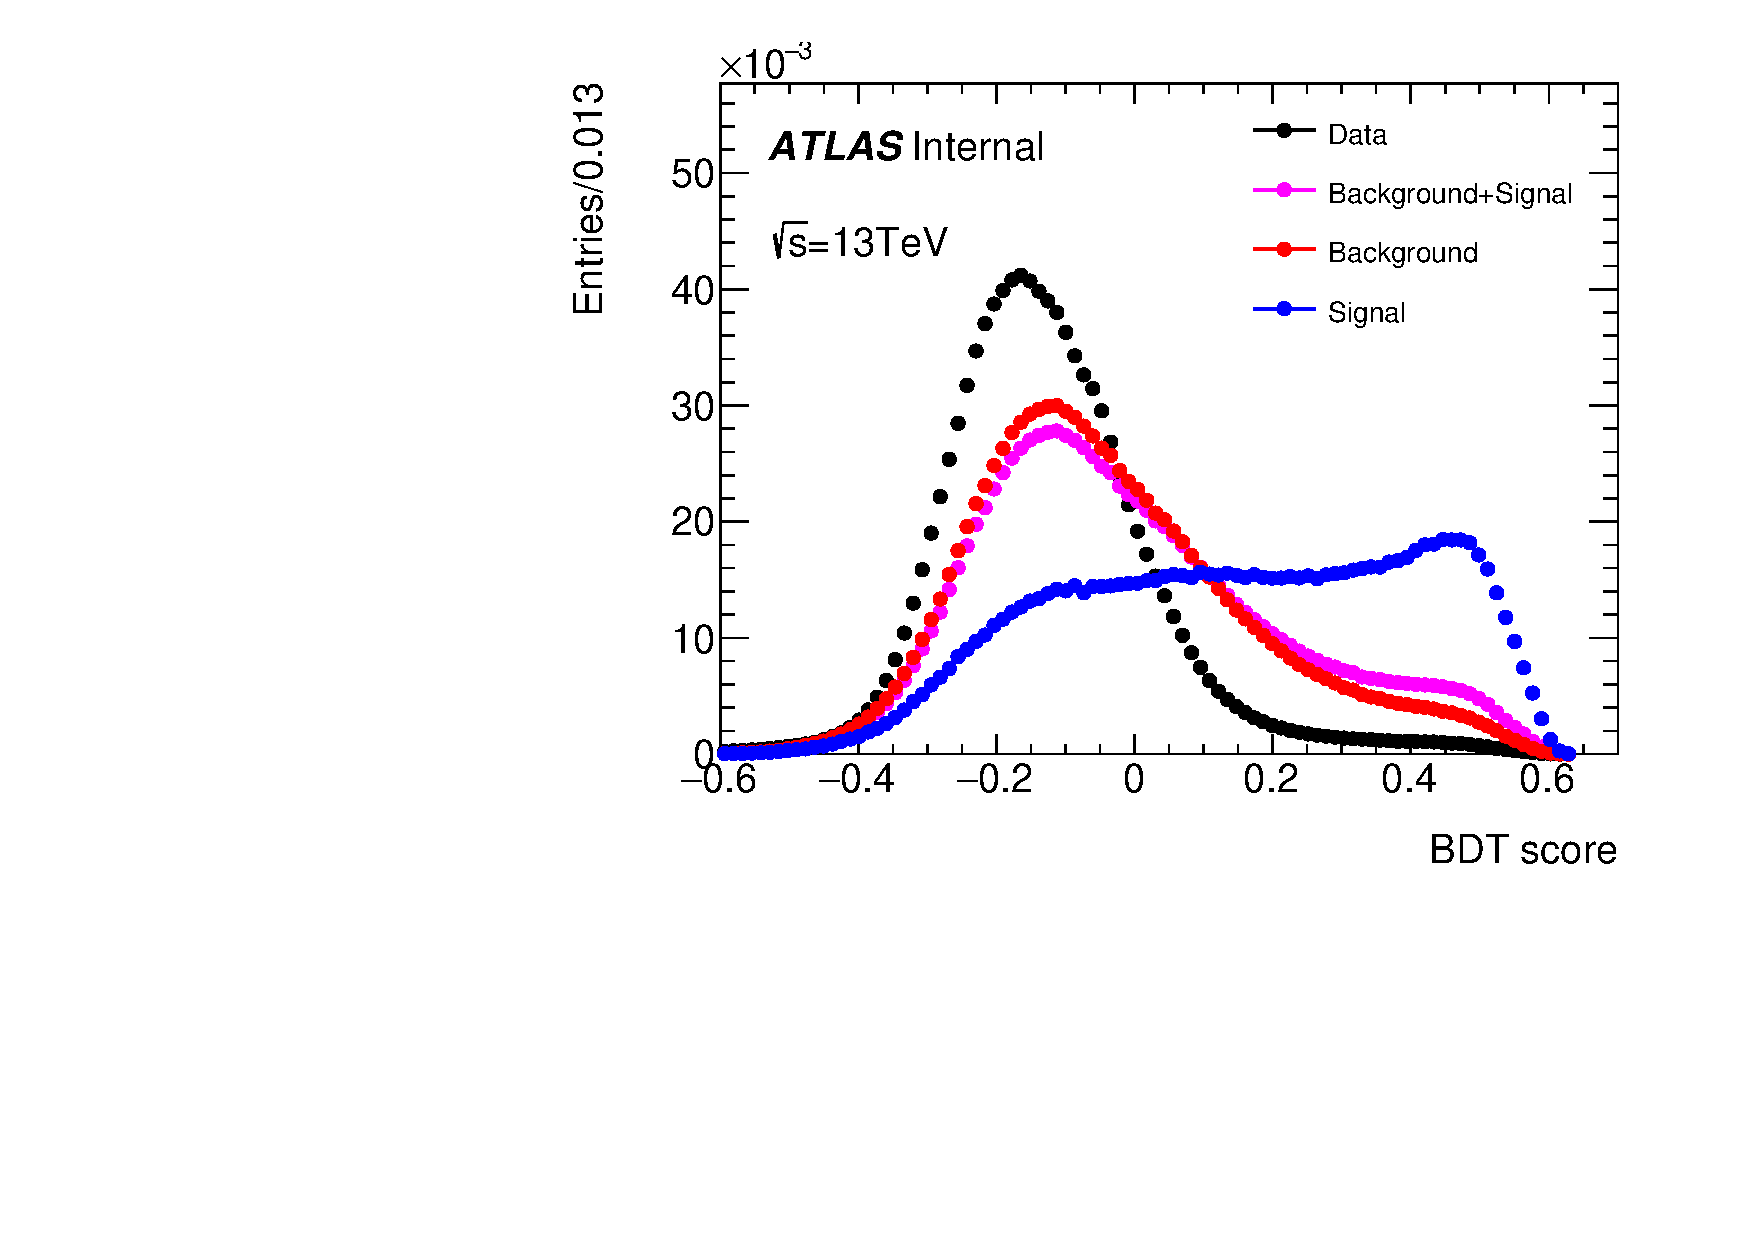
\includegraphics[width=0.45\textwidth]{BDT_Wide.pdf}
    }
    \subfloat[]
    {
	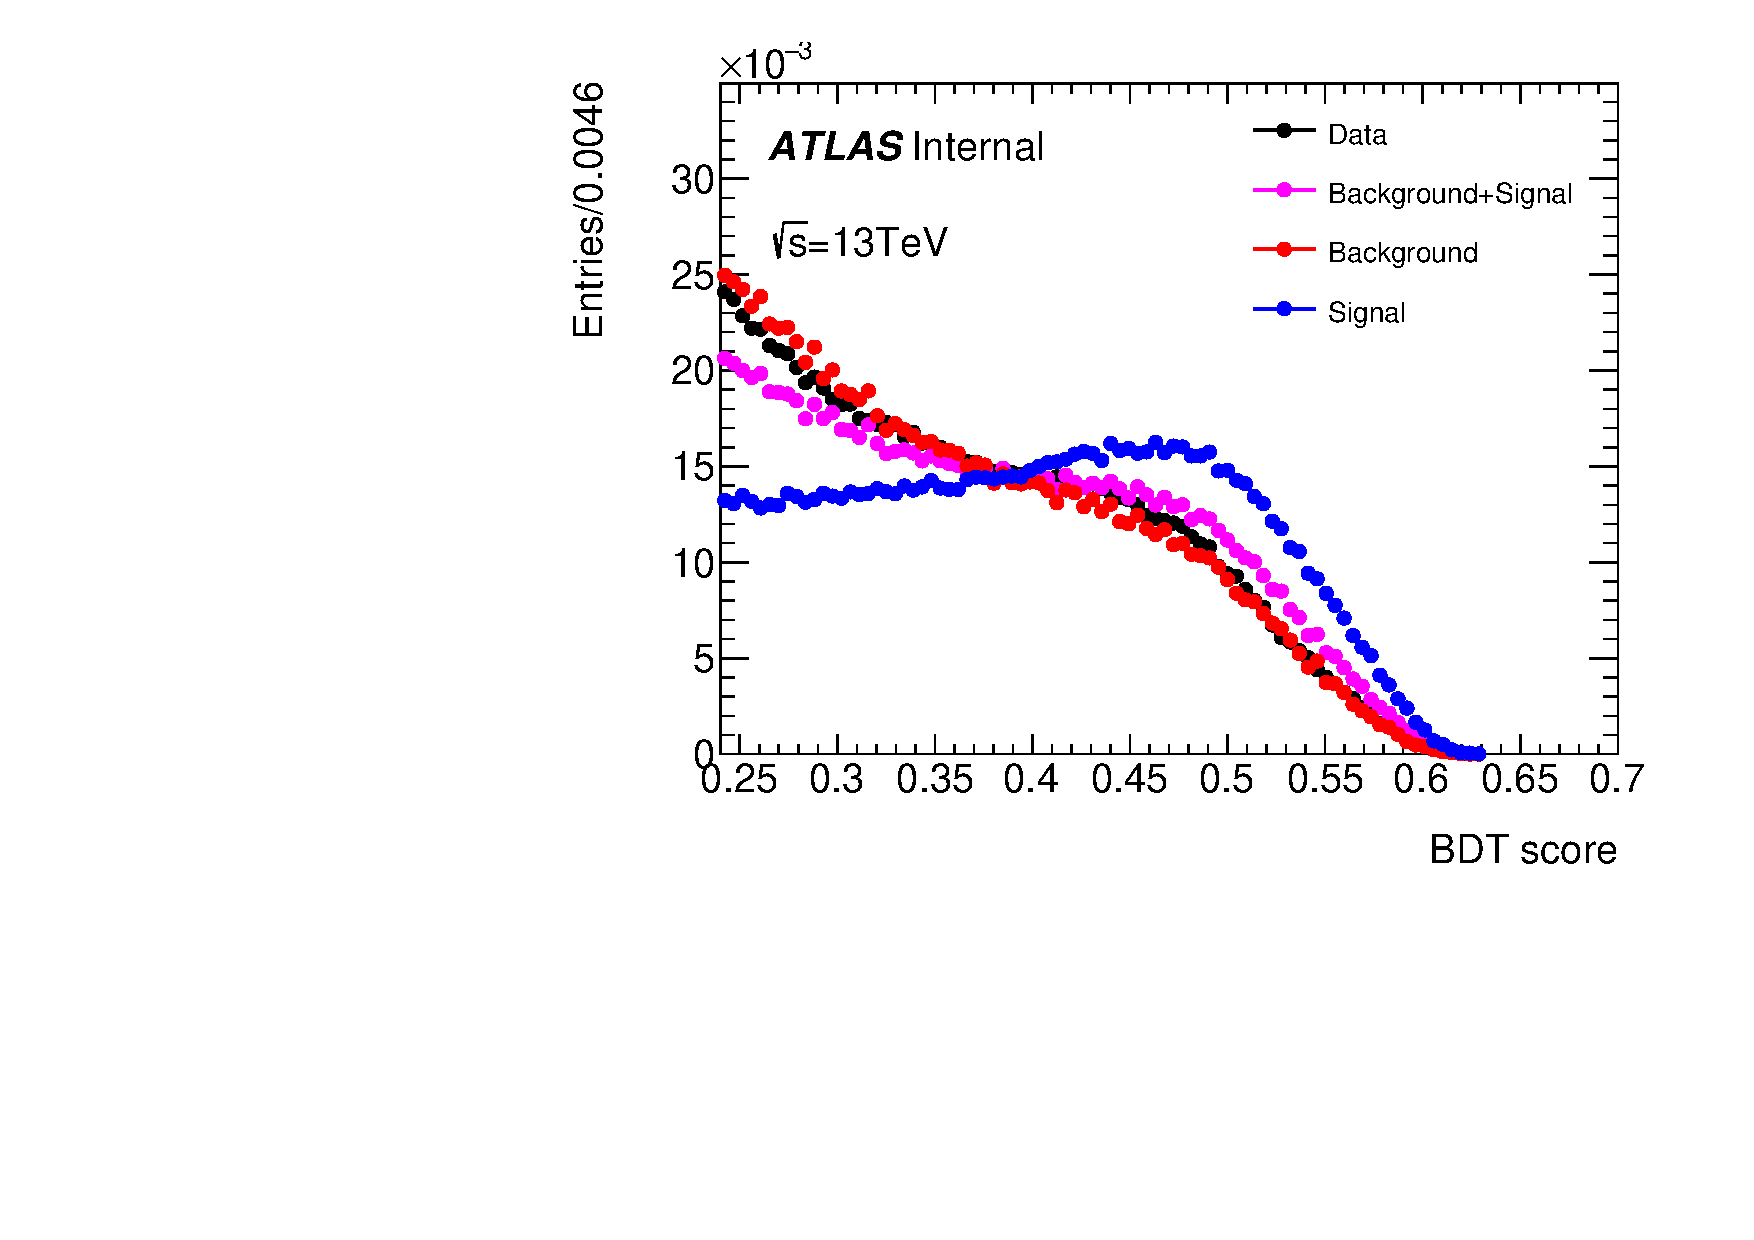
\includegraphics[width=0.45\textwidth]{BDT_Narrow.pdf}
    }
    \caption{BDT score distribution for signal MC, background and data.}
    \label{fig:bplus_bdt_score}
\end{figure}

The background was extracted from the $\bbjpsix$ sample, after the signal component was filtered out.
The cutflow for the three samples can be seen in figure \ref{fig:bplus_fit_cutflow}.

\begin{figure}[ht]
    \centering
    \subfloat[Background]
    {
	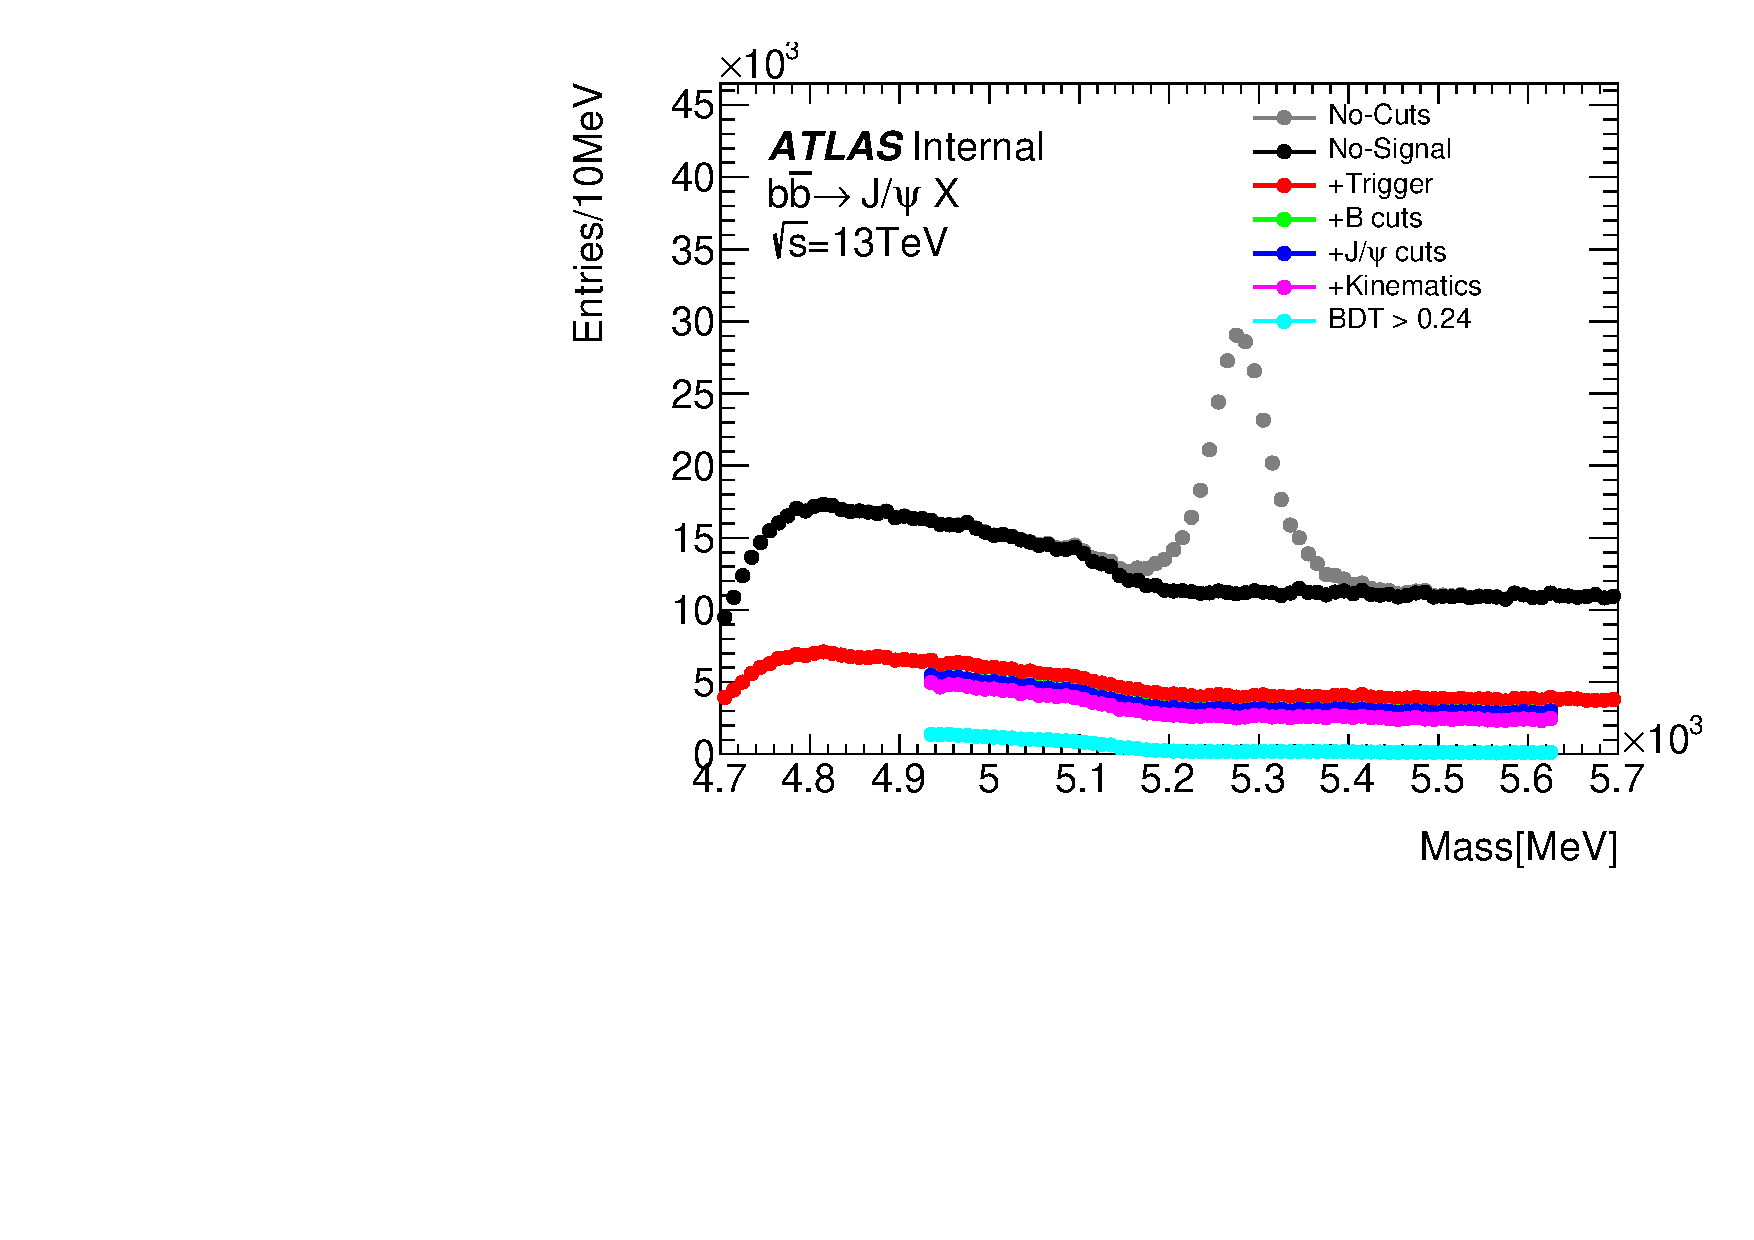
\includegraphics[width=0.45\textwidth]{B_VTX_mass_background.pdf}
    }
    \subfloat[Signal]
    {
	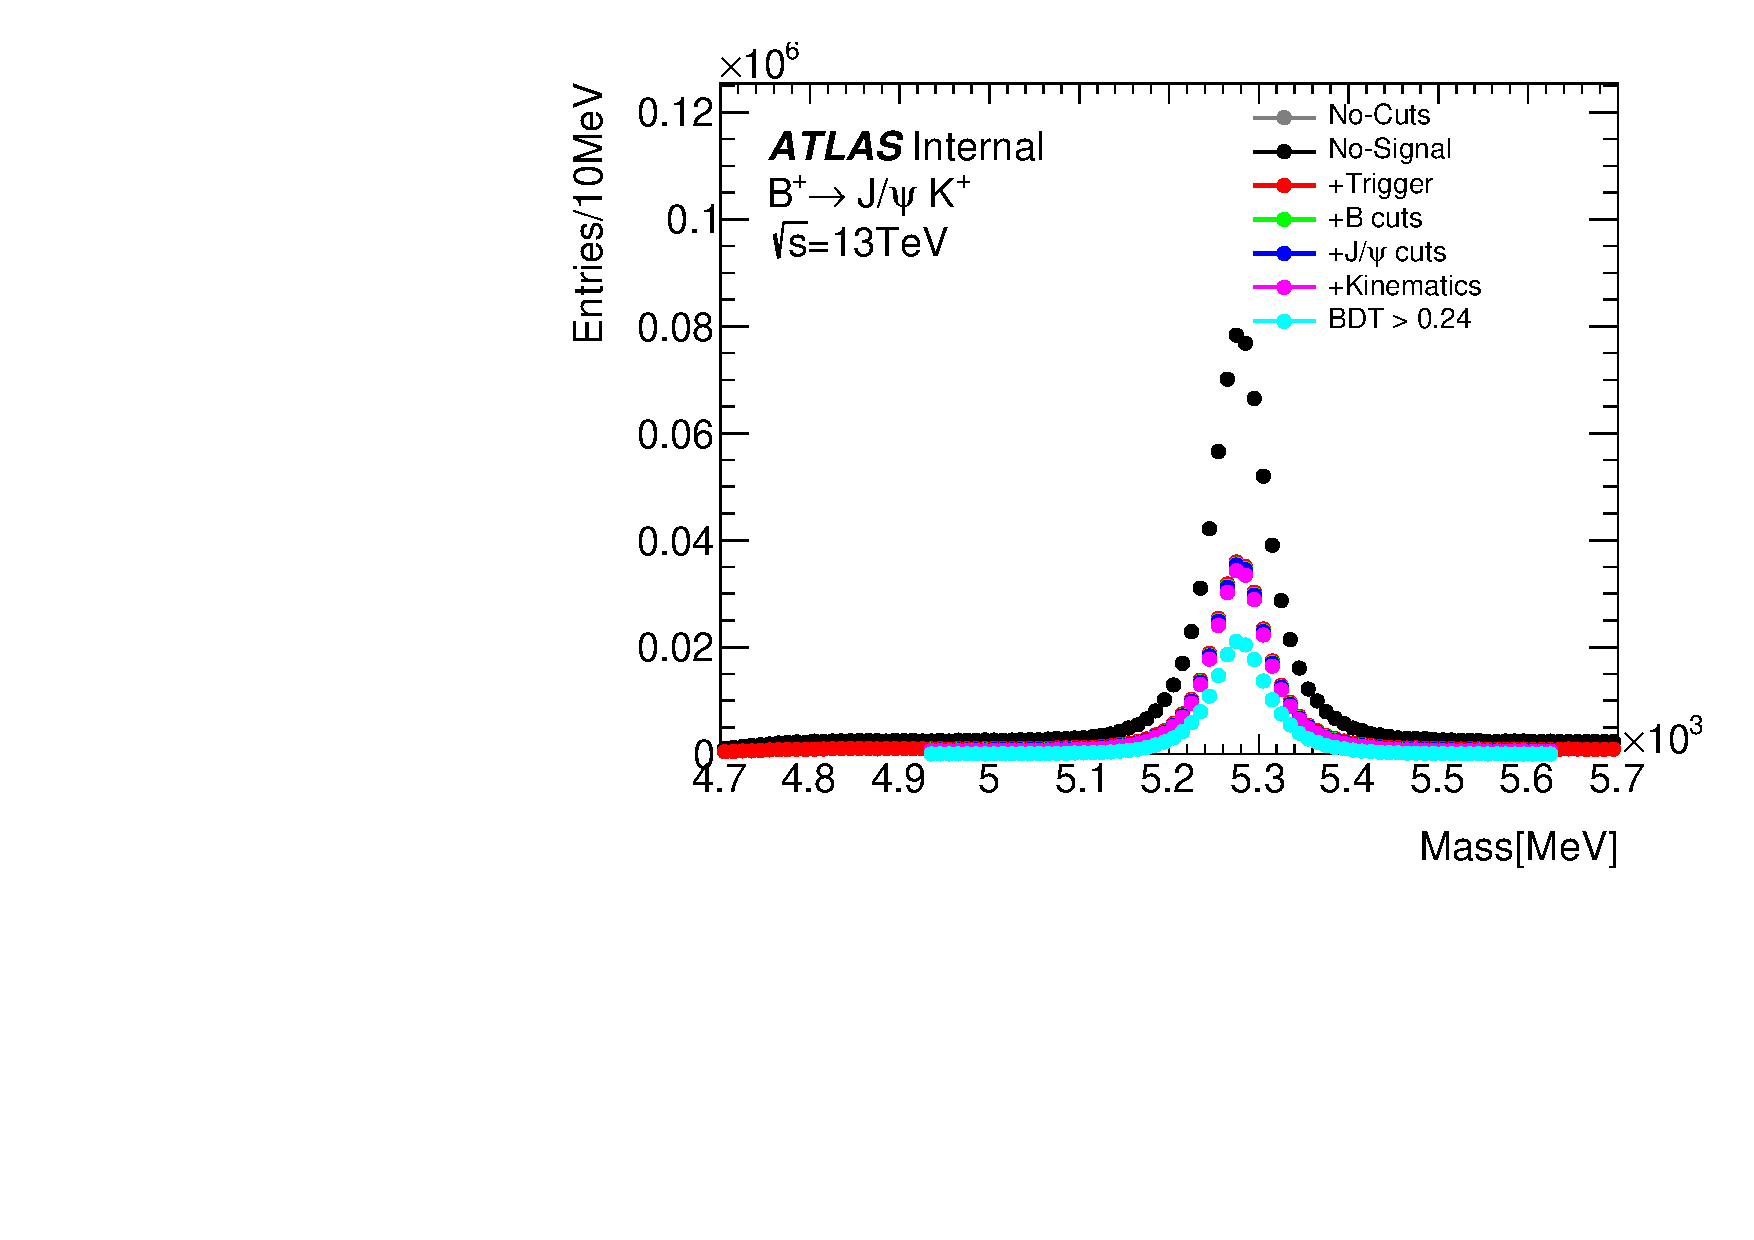
\includegraphics[width=0.45\textwidth]{B_VTX_mass_signal.pdf}
    }

    \subfloat[Data]
    {
	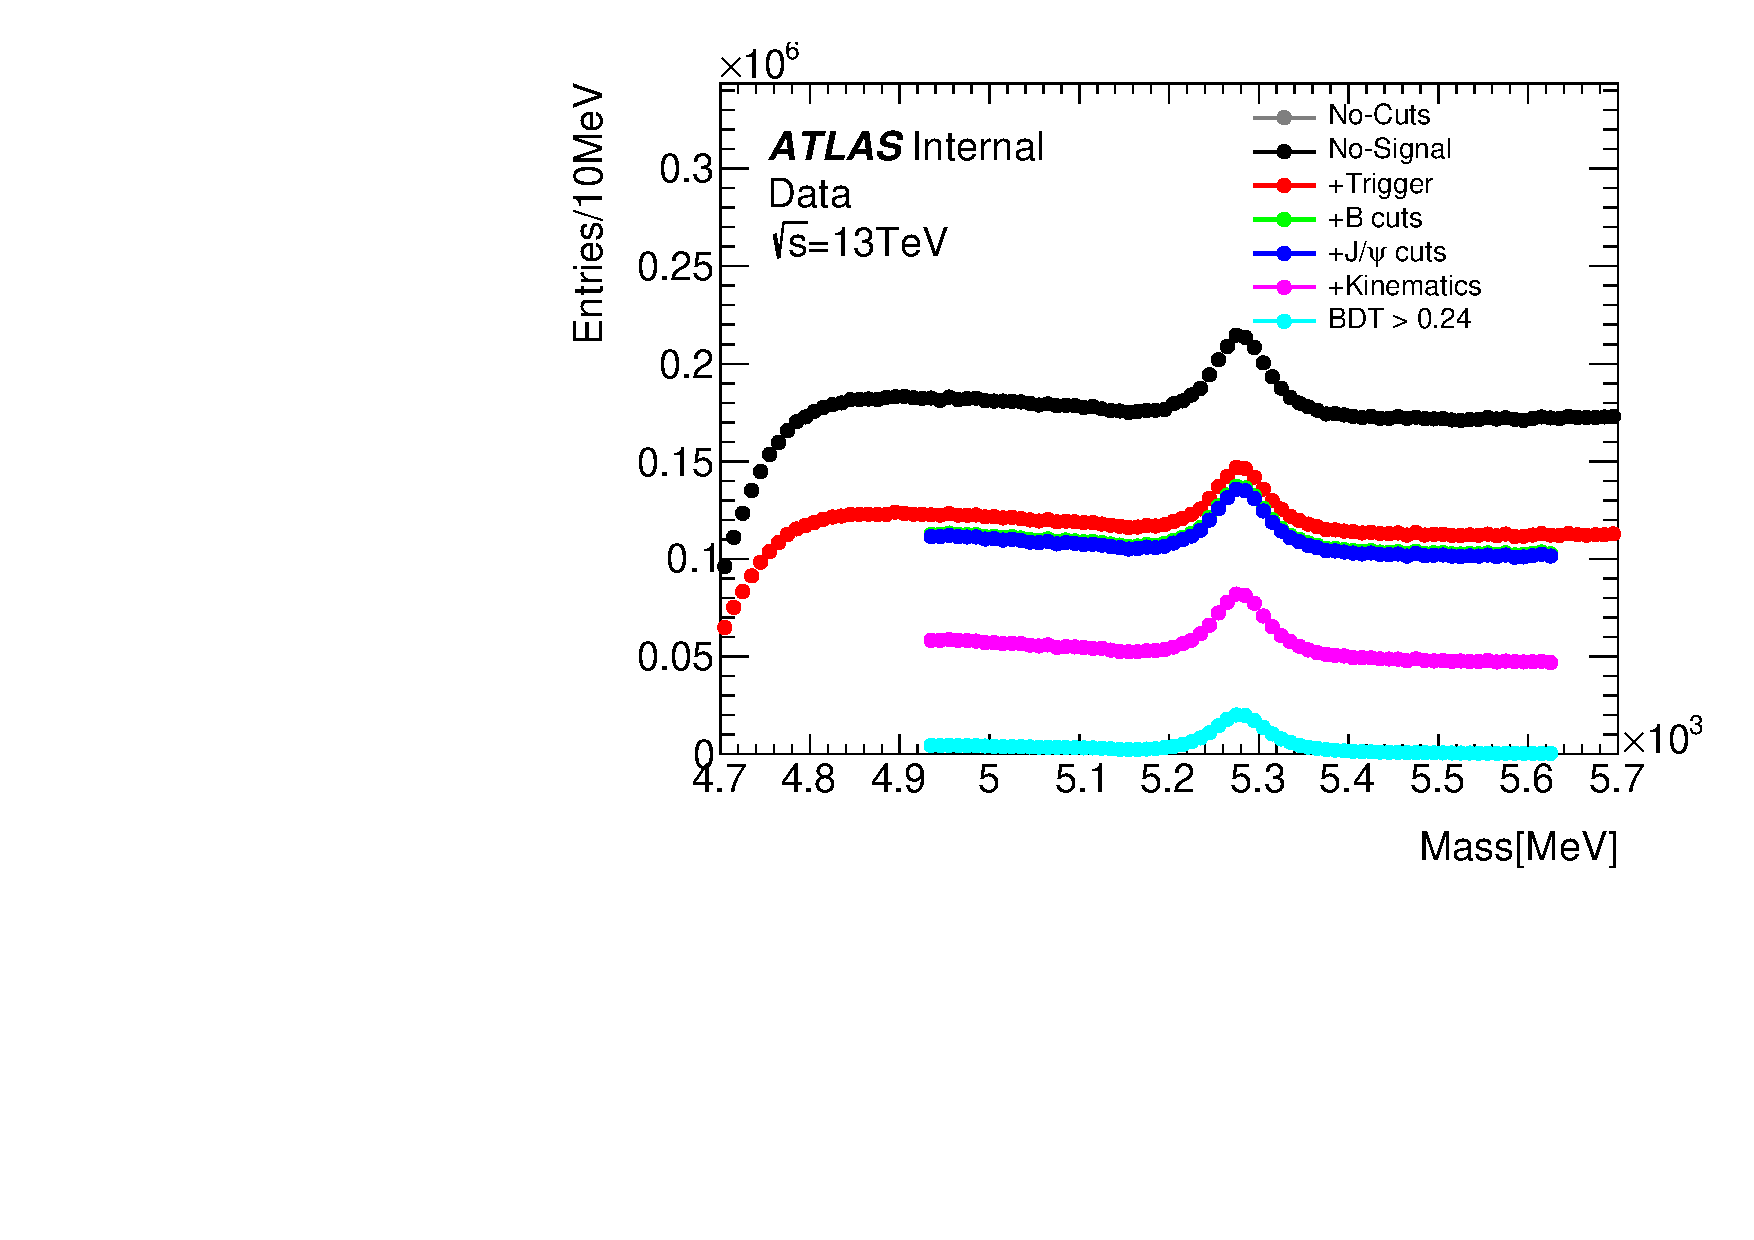
\includegraphics[width=0.45\textwidth]{B_VTX_mass_data.pdf}
    }
    \caption{Cutflow associated to the simulated $\bsmumu$ and $\bpjpsik$ samples, and for the data.}
    \label{fig:bplus_fit_cutflow}
\end{figure}

In these figures \textit{No signal} implies removing the $\bpjpsik$ component
from the respective sample, this obviously only makes sense for the $\bbjpsix$ sample,
otherwise it has no effect. The corresponding efficiencies are in tables \ref{tbl:bplus_cutflow_eff_background},
\ref{tbl:bplus_cutflow_eff_signal} and \ref{tbl:bplus_cutflow_eff_data}. After applying 
this selection the background composition is as shown in table \ref{tbl:bplus_bckg_selection}.

\begin{table}[ht]
    \centering
    \begin{tabular}{| l | c | r |}
	\hline
	Cut   & Efficiency & Number of Events\\ 
	\hline
	No Signal & 0.91 & 1695814\\ 
	Trigger & 0.37 & 629375\\ 
	Cuts on B & 0.15 & 251257\\ 
	Cuts on $J/\psi$ & 0.15 & 249617\\ 
	Cuts on kinematic quantities & 0.13 & 215851\\ 
	BDT & 0.02 & 31101\\ 
	\hline
    \end{tabular}
    \caption{Cutflow efficiency for $\bbjpsix$ sample.}
    \label{tbl:bplus_cutflow_eff_background}
\end{table}

\begin{table}[ht]
    \centering
    \begin{tabular}{| l | c | r |}
	\hline
	Cut   & Efficiency & Number of Events\\ 
	\hline
	No Signal & 1.00 & 990211\\ 
	Trigger & 0.43 & 429273\\ 
	Cuts on B & 0.36 & 353872\\ 
	Cuts on $J/\psi$ & 0.35 & 351176\\ 
	Cuts on kinematic quantities & 0.34 & 335628\\ 
	BDT & 0.19 & 188707\\ 
	\hline
    \end{tabular}
    \caption{Cutflow efficiency for $\bpjpsik$ sample.}
    \label{tbl:bplus_cutflow_eff_signal}
\end{table}

\begin{table}[ht]
    \centering
    \begin{tabular}{| l | c | r |}
	\hline
	Cut   & Efficiency & Number of Events\\ 
	\hline
	No Signal & 1.00 & 23470163\\ 
	Trigger & 0.66 & 15553565\\ 
	Cuts on B & 0.33 & 7691019\\ 
	Cuts on $J/\psi$ & 0.32 & 7602035\\ 
	Cuts on kinematic quantities & 0.16 & 3860800\\ 
	BDT & 0.01 & 292550\\ 
	\hline
    \end{tabular}
    \caption{Cutflow efficiency for data.}
    \label{tbl:bplus_cutflow_eff_data}
\end{table}

\begin{table}[ht]
    \centering
    \begin{tabular}{| l | r |}
	\hline
	Frequency & Decay\\ 
	\hline
	11015 & B0[K*0[pi-:K+]J/psi[mu+:mu-]] \\ 
	7797 & unmatched \\ 
	3598 & B+[K*+[pi0[gamma:gamma]K+]J/psi[mu+:mu-]] \\ 
	1750 & B+[K+:chi\_1c[gamma:J/psi[mu+:mu-]]] \\ 
	1411 & B+[pi+:J/psi[mu+:mu-]] \\ 
	751 & B0[K*0[pi-:gamma:K+]J/psi[mu+:mu-]] \\ 
	471 & B0[pi-:K+:J/psi[mu+:mu-]] \\ 
	442 & B+[rho+[pi0[gamma:gamma]pi+]J/psi[mu+:mu-]] \\ 
	278 & B0[K*\_20[pi-:K+]J/psi[mu+:mu-]] \\ 
	252 & B+[K*+[pi+:K0[K\_S0]]J/psi[mu+:mu-]] \\ 
	250 & B+[K*+[pi+:K0[K\_L0]]J/psi[mu+:mu-]] \\ 
	239 & combinatorial \\ 
	214 & B+[pi0[gamma:gamma]K+:J/psi[mu+:mu-]] \\ 
	191 & B0[rho0[pi-:pi+]J/psi[mu+:mu-]] \\ 
	187 & B+[gamma:pi+:J/psi[mu+:mu-]] \\ 
	149 & B\_s0[pi-:pi+:J/psi[mu+:mu-]] \\ 
	135 & B\_s0[eta'[gamma:rho0[pi-:pi+]]J/psi[mu+:mu-]] \\ 
	118 & B+[gamma:K*+[pi0[gamma:gamma]K+]J/psi[mu+:mu-]] \\ 
	118 & B+[K+:chi\_0c[gamma:J/psi[mu+:mu-]]] \\ 
	102 & B+[K*\_2+[pi0[gamma:gamma]K+]J/psi[mu+:mu-]] \\ 
	89 & B*-[B-[K-:J/psi[mu+:mu-]]gamma] \\ 
	81 & missing particles \\ 
	79 & B+[gamma:K+:chi\_1c[gamma:J/psi[mu+:mu-]]] \\ 
	76 & B+[K*\_2+[pi+:K0[K\_L0]]J/psi[mu+:mu-]] \\ 
	76 & B+[K*\_2+[pi+:K0[K\_S0]]J/psi[mu+:mu-]] \\ 
	69 & B+[pi+:K0[K\_L0]J/psi[mu+:mu-]] \\ 
	52 & B+[pi+:K0[K\_S0]J/psi[mu+:mu-]] \\ 
	41 & B+[K*+[pi0[e+:e-:gamma]K+]J/psi[mu+:mu-]] \\ 
	39 & Xi\_b+[Xi-\_bar:J/psi[mu+:mu-]] \\ 
	\hline
    \end{tabular}
    \caption{Background composition of $\bbjpsix$ sample selection is applied.}
    \label{tbl:bplus_bckg_selection}
\end{table}

Additionally figure \ref{fig:decay_distribution} shows the distribution of the number of decays
versus the index of the decay, when the most common decays are put at the beginning, the plot
also shows the corresponding cumulative distribution.

There are 81 candidates classified as \textit{missing particle} for which the matching is not possible
given that there are no particles in the event record, that follow the requirements. 

\begin{figure}
    \centering
    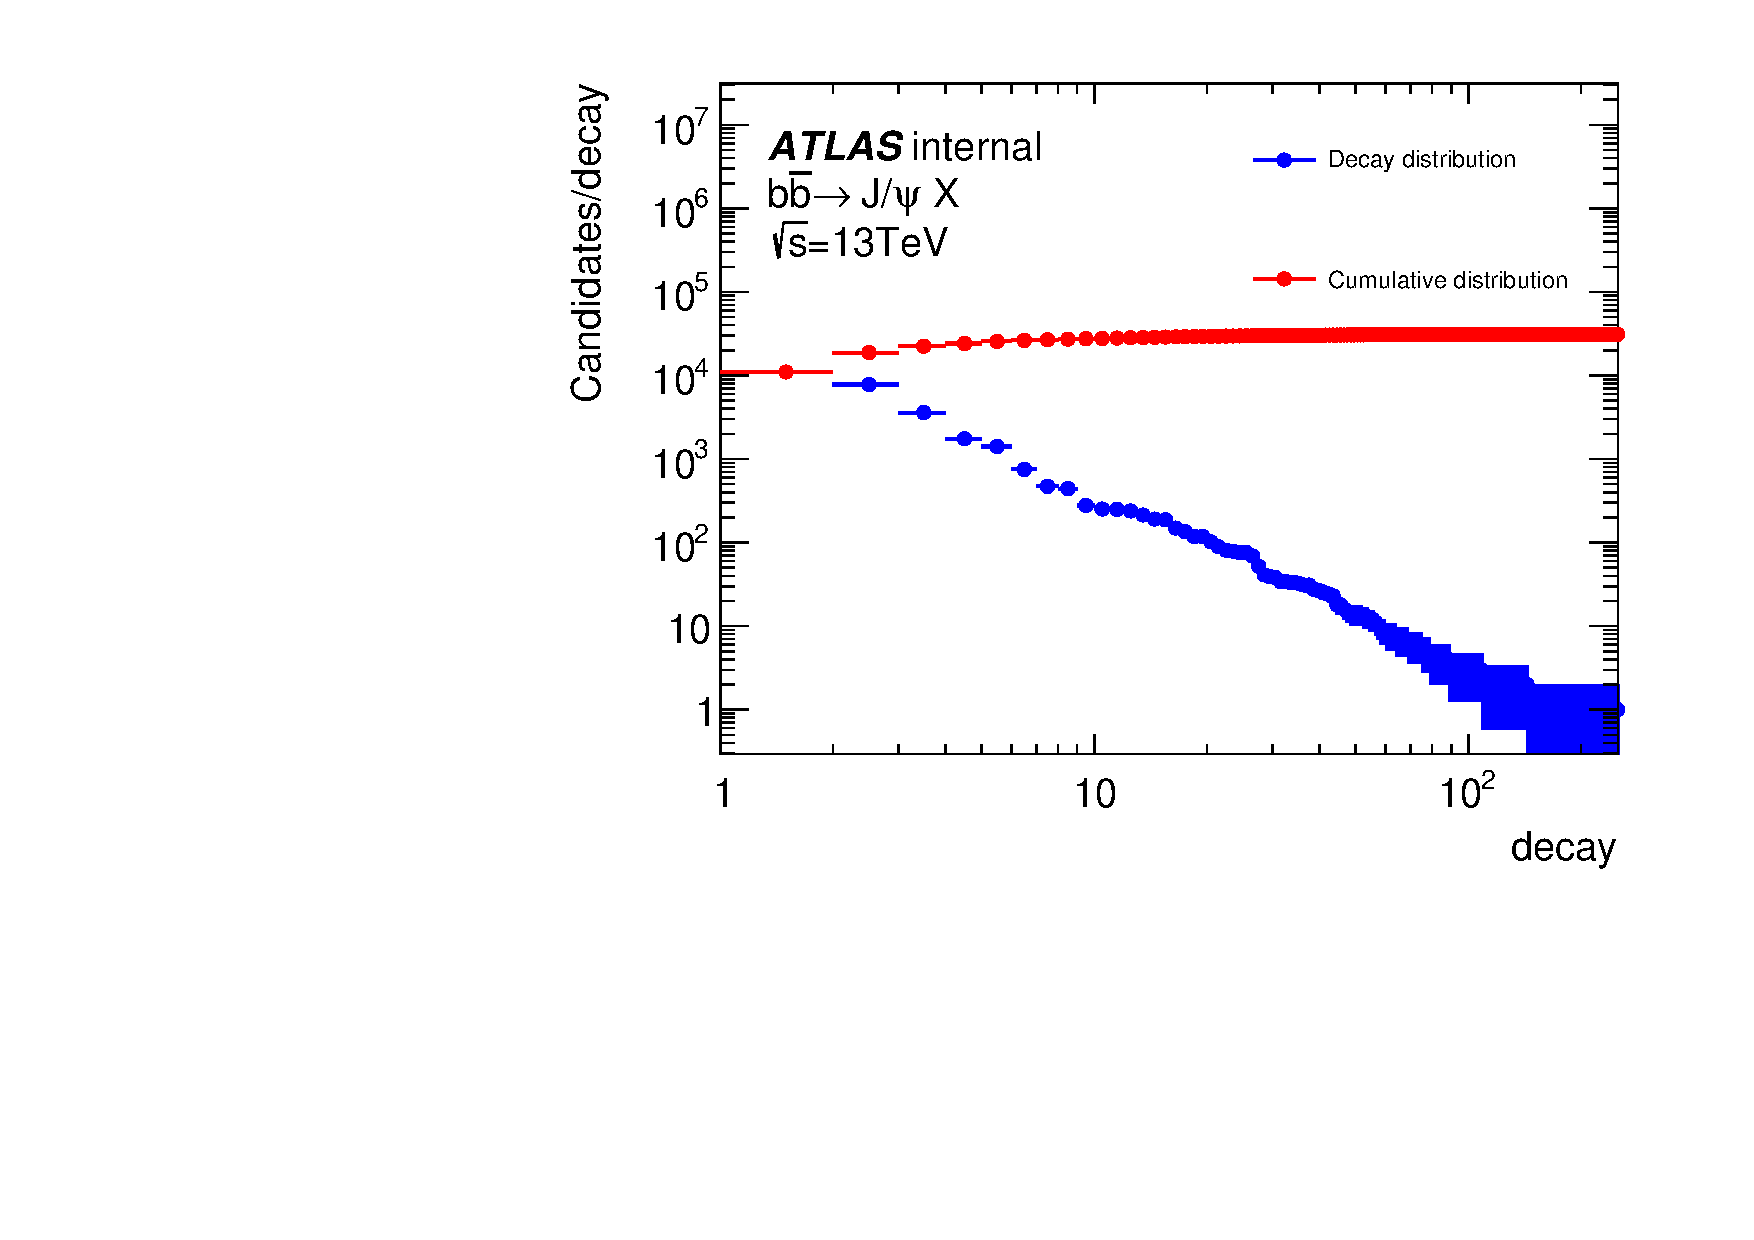
\includegraphics[width=0.70\textwidth]{decay_frequency.pdf}
    \caption{Decay distribution and the corresponding cumulative distribution.}
    \label{fig:decay_distribution}
\end{figure}

\subsection{Procedure}
To extract the $B^+$ yield for the reference channel, we use a
unbinned maximum likelihood fit to the mass distribution.
The fit is performed simultaneously on data and the MC samples
from which the models are taken.
With respect to the 2011 analysis, the event-by-event error is
no longer used as it provides very limited or no separation.

\begin{figure}[!htb]
    \begin{center}
	\hspace{-0.5cm}
	
\includegraphics[width=0.52\textwidth]{dataonlyN3.eps}
	\hspace{-0.5cm}
	
\includegraphics[width=0.52\textwidth]{mcprdN3.eps}
	\caption{{\it Left}: $J/\psi K^{\pm}$ invariant mass distribution for all $B^{\pm}$
	    candidates in 2012 data.
	    {\it Right}: partially reconstructed $B$ decays contributing to the background
	as described by Monte Carlo.}
	\label{fig:bplusinvmass}
    \end{center}
\end{figure}

In the $B^\pm$ invariant mass distribution (shown in Figure~\ref{fig:bplusinvmass},
left plot) the $B^\pm$ signal is quite evident, but with visible contributions
from at least three background categories. On the left of the $B^\pm$ peak
we find the partially reconstructed $B$ decays
(PRD, e.g. $B^{+/0} \to K^{*+/0} J/\psi$, $B^{+} \to K^{+} \chi_{c1,2}$) 
where one or more of the final state particles are missed in the reconstruction.
On the right side, it is expected a contribution from the reflection of the
Cabibbo-suppressed $B^\pm\to J/\psi\pi^\pm$ decay with the assignment of the
kaon mass to the final state pion.
Finally there is the combinatorial background, which MC studies suggest to be composed,
after our selection cuts, mostly of $b\bar{b}\to \jpsi X$ that spans on the whole mass
range, and consists of random combination of \jpsi\ (produced promptly in $pp$ collisions
or in feed-down from B-decays) with a track.

For the extraction of the $B^+$ yield, we define the following event categories:
\begin{itemize}
    \setlength{\itemsep}{0pt}%
	\setlength{\parskip}{0pt}%
    \item \NJpsiK{}: number of \BpmKpmJpsi{} events (signal events for this fit);
    \item \NJpsipi{}: number of \BpPipJpsi{} events;
    \item \Npr{}: number of partially reconstructed events (PRD);
    \item \Nc{}: number of combinatorial events.
\end{itemize}

Table~\ref{tab:fit_candidates} shows the \BpmKpmJpsi{} candidates, in the mass region
$4930-5630\ \mathrm{MeV}$, passing the complete selection (including the final
continuum BDT cut). 

\begin{table}[!htb]
    \begin{center}
	%input{appendix/bplusfit_table_data.tex}
	\label{tab:fit_candidates}
    \end{center}
\end{table}

The fit is based on a unbinned extended maximum likelihood fit to data
with simultaneous inclusion of three MC samples to guide the modeling of
several fit components.
The MC samples are introduced to model accurately the shapes of the \BpmKpmJpsi{} 
events as well as the most critical background components: the PRD and the
$J/\psi\pi^\pm$ decays.
By fitting the above mentioned MC samples simultaneously, we constrain the
fit parameters of the corresponding fit components to their MC values.
This results in an \textit{MC assisted} determination of the background shapes,
while automatically accounting for the statistical uncertainties of the MC.
Two free parameters, one for the mass scale and the other for the mass resolution
are extracted from data to accommodate for the possible data-MC difference
in the shapes for \BpmKpmJpsi{}, PRD and $J/\psi\pi^\pm$ decays.

The probability density functions (PDF's) used in this fit are described
below. The parameters of each function are tied among the data and MC samples,
so that effectively the parameter values that are determined by the fit
on the MC components are propagated to functions used to fit the data
components.

The three MC samples included in the simultaneous fit are:
\begin{itemize}
    \setlength{\itemsep}{0pt}%
	\setlength{\parskip}{0pt}%
    \item \BpmKpmJpsi{} MC events: $B^+\to J/\psi K^+$ ($J/\psi\to\mu^+\mu^-$)
	exclusively generated. These events include also radiative decays where
	the $B^\pm$ radiates a $\gamma$. The two cases are modeled separately in
	the fit but they are both included in the signal definition.
    \item $B^\pm\to J/\psi\pi^\pm$ MC: used to describe this reflection when the
	$K$ mass is mis-assigned to the final state pion.
    \item $bb\to J/\psi X$ MC sample: PRD events are characterized by this sample.
	Where we can distinguish the true origin of each reconstructed
	$B^\pm$ candidate. In order to model the PRD contribution to the mass fit,
	we identify three classes of decays contributing with slightly different mass shapes.
	The three classes are as follows:
	\begin{itemize}
	    \item PRD1: these events produce a step shape at 5150 MeV:
		these are mainly
		$B^0\rightarrow J/\psi  K^{*0}$,
		$B^+\rightarrow J/\psi  K^{*+}$,
		$B^0\rightarrow J/\psi  \rho^{0}$,
		$B^+\rightarrow J/\psi  \rho^{+}$,
		$B^0\rightarrow J/\psi  K^+\pi^-$, and
		$B^+\rightarrow J/\psi  K^+\pi^{0}$.
	    \item PRD2: these events produce a bump at 5050 MeV.
		These events are mainly 
		$B^+\rightarrow\chi_{c1}K^+$.
		%and $B^+\rightarrow \chi_{c2}K^+$.
	    \item PRD3: this component includes everything else
		from the $J/\psi X$ sample and has a smoother shape
		in the mass distribution.
	\end{itemize}
\end{itemize}

The PDF's used are the following:
\begin{itemize}
    \setlength{\itemsep}{0pt}%
	\setlength{\parskip}{0pt}%
    \item \BpmKpmJpsi{} signal:
	Johnson $S_U$~\cite{Johnson}, this PDF contains the core of the signal events and
	it is parameterized as follows:
	\begin{equation}
	    \mathrm{Johnson}~S_U =
	    \frac{1}{\sqrt{1+t^2}}\left[t+\sqrt{1+t^2}\right]^{-\gamma-\frac{1}{2}\delta\ln{(t+\sqrt{1+t^2})}} \text{, where } t = \frac{m-\xi}{\lambda}
	\end{equation}
	where $\xi = s_\mu + \xi^{MC}$ in which $s_\mu$ parameterizes the
	possible mass scale shift between data and MC. The same $s_\mu$
	scale shift is applied to the Gaussian mean: $s_\mu+\mu^{MC}$ where
	$\mu^{MC}$ is the mean of the Gaussian shape in the \BpmKpmJpsi{} MC sample.
	Parameters $\lambda$, $\xi$, $\delta$ and $\gamma$ determine the shape
	of the distribution Johnson $S_U$ distribution. The parameters $\xi$
	and $\lambda$ control the position and width of the distribution,
	respectively. The sign of $\gamma$ determines the position of
	the tail (left or right to the peak).

	A data-MC discrepancy is allowed also in the resolution parameters:
	the Johnson $S_U$ distribution is convoluted with a Gaussian resolution function
	with zero mean and $s_\sigma$ width where the latter parameter describes 
	the resolution difference between data and MC.
	The same effect is taken into account in the Gaussian distribution
	whose width is thus obtained by summing in quadrature the MC width
	$\sigma^{MC}$ and the resolution smearing factor $s_\sigma$.

	The model of the shape is taken from \BpmKpmJpsi{} MC events
	and its parameters are left floating in the fit to be determined from
	the \BpmKpmJpsi{} MC sample in the simultaneous fit.
	The normalization and the $2$ scaling factors allow the distribution to
	adjust to the data peak.
	Details on the specific implementation of these parameterizations
	are found in Appendix~\ref{app:sec:bplusfitsigdescription}.

    \item radiative contribution to \BpmKpmJpsi{} decays: when the $B$ radiates a $\gamma$,
	the mass shape results skewed on the left so we need to consider
	this component separately. A single Johnson $S_U$ is used. 

	The shape parameters are determined from the radiative decays selected
	in the $J/\psi K^\pm$ MC sample.
	The normalization and the $2$ scaling factors allow the distribution to
	adjust to the data peak.
	Details on the specific implementation of these parameterizations
	are found in Appendix~\ref{app:sec:bplusfitsigdescription}.

	The relative abundances of the two signal components (non-radiative
	and radiative) are parametrized using relative fractions so that
	the total number of \BpmKpmJpsi{} events is extracted from the fit
	together with the three fractions.

    \item $J/\psi\pi^\pm$ final states:
	similarly to the \BpmKpmJpsi{} component, a Johnson $S_U$. 
	Also in this case the shape parameters are determined
	from the $J/\psi\pi^\pm$ MC sample in the simultaneous fit.

	The $2$ overall scaling factors on the mass scale and resolution
	are also applied to these parameterizations: in the fit they are
	driven by the effect on the \BpmKpmJpsi{} component.

    \item PRD component:
	\begin{itemize}
	    \setlength{\itemsep}{0pt}%
		\setlength{\parskip}{0pt}%
	    \item PRD1 with 5150-step shape.
		We parameterize these events with a Fermi-Dirac (FD) plus an Exponential
		The FD distribution is parametrize as follows:
		\[
		    \mathrm{M_{FD}}(m|\mu_{FD}, \alpha_{FD})=\frac{1}{1+e^{\frac{m - \mu_{FD}}{\alpha_{FD}}}}
		\]
		where $\alpha_{FD}$ accounts for the slope, while $\mu_{FD}$ accounts for
		the mass scale at which the step-like effect occurs.
		The shape parameters are taken from the PRD1 events in the
		$(bb\to\mu^-\mu^+X)_{\mathrm{pr}}$ MC sample in the simultaneous fit.
		In the parameterization used for data the FD mass scale parameter $\mu_{FD}$
		is redefined as $\mu^{MC}_{FD} + s_\mu$ where $s_\mu$ is the scale factor
		already defined above and it is common to the \BpmKpmJpsi{} and $J/\psi\pi^\pm$ events.
		The PDF is then convoluted with the Gaussian resolution function
		with the $s_\sigma$ width already defined above and common to the \BpmKpmJpsi{}
		and $J/\psi\pi^\pm$ events.

	    \item PRD2 with 5000-bump shape.
		We parameterize these events with a FD plus an Exponential
		Again the $2$ overall scaling factors on
		the mass scale and resolution are applied to these parameterizations.
		The shape parameters are taken from the PRD2 events in the
		$(bb\to\mu^-\mu^+X)_{\mathrm{pr}}$ MC sample in the simultaneous fit.

	    \item PRD3 with a falling shape.
		We parameterize these events with an Exponential plus a constant term.
		Again the $2$ overall scaling factors on
		the mass scale and resolution are applied to these parameterizations.
		The shape parameters are taken from the PRD3 events in the
		$(bb\to\mu^-\mu^+X)_{\mathrm{pr}}$ MC sample in the simultaneous fit.

	\end{itemize}
	Details on the specific implementation of these parameterizations
	are found in Appendix~\ref{app:sec:bplusfitPRDdescription}.
	The relative abundances of the PRD three components are taken from 
	the MC predictions, while the PDG values of these are used as a
	systematic check.
	The total number of PRD events is extracted from the data fit.

    \item combinatorial background:
	exponential function
	\[
	    \mathrm{M_{c}}(m|a)=e^{a m}
	\]
	with the shape parameter that is left floating in the fit
	to be extracted from data.
\end{itemize}

Figures~\ref{fig:bplusfitN12} and~\ref{fig:bplusfitN32011} show the results of the fits: 
the projection on the \Bp\ mass are shown for data.
Appendix~\ref{app:bplusfits} contains the complete fit results including the 
projections on the mass for the MC samples.
As an example, we show in Figure~\ref{fig:bplusfitN3all} all the simultaneous fit results. 
Table~\ref{tab:bplusfit3pars} shows the parameters from the fit, 
again as an example. In Appendix~\ref{app:bplusfits} similar
tables are shown.

\clearpage
\begin{figure}[!htb]
    \begin{center}
	
\includegraphics[width=0.52\textwidth]{datafitN2.eps}
	\caption{Fit projection on 
	    The red line represents the \BpmKpmJpsi{} signal (including both radiative
	    and non-radiative components), while the magenta line represents the
	    $J/\psi\pi$ peaking component. The blue line shows all the three partially
	    reconstructed contributions and the green line represents the
	    combinatorial background. The total of all functions is presented
	with the black line.}
	\label{fig:bplusfitN12}
    \end{center}
\end{figure}

\begin{figure}[!htb]
    \begin{center}
	\hspace{-0.5cm}
	
\includegraphics[width=0.52\textwidth]{datafitN3.eps}
	\hspace{-0.5cm}
	
\includegraphics[width=0.52\textwidth]{datafitN2011.eps}
	\caption{Fit projection on data (left) and for the 2011 data (right).
	    The red line represents the \BpmKpmJpsi{} signal (including both radiative
	    and non-radiative components), while the magenta line represents the
	    $J/\psi\pi$ peaking component. The blue line shows all the three partially
	    reconstructed contributions and the green line represents the
	    combinatorial background. The total of all functions is presented
	with the black line.}
	\label{fig:bplusfitN32011}
    \end{center}
\end{figure}

\begin{figure}[!htb]
    \begin{center}
	\hspace{-0.5cm}
	
\includegraphics[width=0.40\textwidth]{mcfitsigN3.eps}
	\hspace{-0.5cm}
	
\includegraphics[width=0.40\textwidth]{mcfitradsigN3.eps}
	\hspace{-0.5cm}
	
\includegraphics[width=0.40\textwidth]{mcfitjpsipiN3.eps}
	\hspace{-0.5cm}
	
\includegraphics[width=0.40\textwidth]{mcfitprd1N3.eps}
	\hspace{-0.5cm}
	
\includegraphics[width=0.40\textwidth]{mcfitprd2N3.eps}
	\hspace{-0.5cm}
	
\includegraphics[width=0.40\textwidth]{mcfitprd3N3.eps}
	\caption{Fit projections on the MC samples simultaneous fitted with the data.
	    From left to right, from top to bottom: non-radiative \BpmKpmJpsi{} signal, 
	    radiative \BpmKpmJpsi{} signal, peaking background $J/\psi \pi$, PRD1, PRD2
	    and PRD3.
	    The red line is used for the \BpmKpmJpsi{} signal (including both radiative
	    and non-radiative components), while the magenta line is for the
	    $J/\psi\pi$ peaking component. The blue lines refer to all the three
	    partially reconstructed contributions.
	    In each plot, the black non-continuous lines show the single functions
	of the total PDF used to model the given component.}
	\label{fig:bplusfitN3all}
    \end{center}
\end{figure}

\clearpage
\begin{table}[!htb]
    \begin{center}
	%input{appendix/bplusfit_table_fitN3.tex}
	\label{tab:bplusfit3pars}.
    \end{center}
\end{table}

\subsection{Systematic Uncertainties in the Extraction of the $B^\pm$ Yields}
\label{sec:bplusyst}

Some of the systematic effects are taken care of automatically in the fit:
the MC effect of limited statistics, for example, is included in the statistical
fit error from the simultaneous fit. In addition the data-MC discrepancy in the
mass scale and resolution is included in the fit using the aforementioned scaling
factors.

Systematic effects on the reference channel yield are coming mainly from the parametrization
of the mass distributions and the data-MC discrepancies. The approximation of mass shapes in the
simultaneous fit by PDFs is a source of systematic uncertainty on the fit result which
we evaluate by repeating the fit varying the fit models. The difference between the modified
and default fit results is then taken as the systematic uncertainty.
The systematic uncertainties can be found in Table~\ref{tab:bplusyst} as
an example. 

The list of systematic checks is the following:
\begin{itemize}
    \setlength{\itemsep}{0pt}%
	\setlength{\parskip}{0pt}%
    \item data-MC discrepancies in $B$ kinematics: discrepancies on the $B$ meson kinematics
	between data and MC introduce a source of uncertainty. GLC- and DDW-weighted $J/\psi K^+$
	and $J/\psi \pi^+$ MC samples account for biases introduced by generator level
	preselection cuts and discrepancies in 2D ($p_{T}$,$\eta$) spectrum of the $B^{\pm}$ with
	respect to data. These reweighted samples are used as alternative MC samples in the simultaneous
	fit.

    \item Alternative model for the PRD3 component: in the PRD3 mass distribution we observe a
	structure not modeled by the Exponential PDF used. We account for this structure by
	adding a Gaussian to the default model.

    \item Combinatorial background model: the combinatorial background smoothly crosses our fit
	window and it is modeled with an exponential function in the default fit. This shape is not
	MC driven. We evaluate the systematic uncertainty coming from the unknown combinatorial
	background model by changing the model to a linear function.

    \item \BpmKpmJpsi{} signal peak charge asymmetry: the MC sample used in the default fit
	is from $B^+ \to J/\psi K^+$ events only. In order to account for shape variations relative to
	$B^- \to J/\psi K^-$, we repeat the fit using the latter.

    \item Alternative models for PRD1 and PRD2 components: systematics from the choice of PRD1
	and PRD2 models are assessed by replacing the principal (default) FD function with
	complementary error function ($\text{Erfc}(m) = \int_m^\infty \mathrm{e}^{-t^2}\,\mathrm{d}t $)
	in each of the two models.

    \item data-MC PRD composition discrepancies: the PRD MC sample has a relative decay modes
	abundances different than what would be expected according to current PDG measurements.
	Different abundances imply different mass shapes: we account for this data-MC shape
	discrepancy by introducing per-event weights derived from the Pythia and PDG differences.
	The weights correct for the MC shapes as well as for the relative abundances of the three
	PRD components. Two additional free parameters take care of the relative PRD fractions:
	these parameters have unit central values and are allowed to vary (via an external Gaussian
	constraint) within the PDG uncertainties on the BRs.

    \item including radiative tails into 2011 fit: When including radiative tails into 2011 fit
	we need to account for MC11-data11 discrepancies and 2011/2012 kinematic differences.
	To address the first issue, we use as alternate fitting sample 2011 MC weighted by the
	appropriate DDW obtained on 2011 data.
	To account for the MC11/MC12 kinematic differences we take the non-radiative $B^+$ candidates
	in the MC12 and the MC11 \BpmKpmJpsi{} signal, reweight both with the appropriate DDW(\&GLC) and obtain
	2011/2012 weights which we can use to reweight our 2012 MC radiative events to 2011 data
	conditions. These weights are also used in assessing the systematic effects from data-MC
	discrepancies in $B$ kinematics (first bullet above) for the 2011 fit.
	In addition, we perform two systematic fits changing the rad/non-rad fractions
	by $50\%$ and we take the largest variation on the result as systematic
	uncertainty.

\end{itemize}

The relative difference on the $B^+$ yields are given in table~\ref{tab:bplusystN3}. 

The main systematic uncertainties on the $B^+$ yield come from the
MC reweighting, the PRD reweighting and the combinatorial background
parametrization. The overall systematic uncertainties result to be
between $0.8-0.9\%$, depending on the data categories, as it is summarized
in Table~\ref{tab:bplusyst}.

\begin{table}[!htb]
    \begin{center}
	%input{appendix/bplusfit_table_systN3.tex}
	\label{tab:bplusystN3}
    \end{center}
\end{table}

\begin{table}[!htb]
    \begin{center}
	%input{appendix/bplusfit_table_syst.tex}
	\label{tab:bplusyst}
    \end{center}
\end{table}

\subsection{$B^{\pm} \rightarrow J\psi K^{\pm}$ yield results}

We measure the $B^{\pm} \rightarrow J\psi K^{\pm}$ reference channel yield with full
systematic uncertainty evaluation in the four measurement categories as shown in
Table~\ref{tab:bplusyieldresults}.

\begin{table}[!htb]
    \begin{center}
	%input{appendix/bplusfit_table_yieldresults.tex}
	\label{tab:bplusyieldresults}.
    \end{center}
\end{table}

\subsection{$J/\psi \pi^{\pm} / J/\psi K^{\pm}$ ratio measurement}
\label{sec:bpluspikratio}

From the fit described above, we extract both the yields for
$B^{\pm} \to J/\psi K^{\pm}$ and $B^{\pm} \to J/\psi \pi^{\pm}$ and
the systematic checks whose results are in Table~\ref{tab:bplusyst}
record the variation on both yields.
\begin{equation}
    \mathrm{R_{\pi/K}} = 
    \frac{N_{J/\psi \pi^{\pm}}\times I^{J/\psi\pi}_{ext}}{N_{J/\psi K^{\pm}}} 
\end{equation}
where the $J/\psi \pi^{\pm}$ yield is corrected by the factor $I^{J/\psi\pi}_{ext}$
explained below. Then we define the ratio:
\begin{equation}
    \rho_{\pi/K} = \frac{\mathcal{BR}(B^{\pm} \to J/\psi \pi^{\pm} )}
    {\mathcal{BR}(B^{\pm} \to J/\psi K^{\pm}) } 
    = \frac{N_{J/\psi \pi^{\pm}}\times I^{J/\psi\pi}_{ext} }{N_{J/\psi K^{\pm}}}\times
    \frac{\epsilon_{J/\psi K^{\pm} }}{\epsilon_{J/\psi \pi^{\pm}}}
    =\mathrm{R_{\pi/K}} \times 
    \left[\frac{\epsilon_{K^{+}}}{\epsilon_{\pi^{+}}} \times 
    \frac{1+\frac{{\epsilon_{K^{-}}}}{\epsilon_{K^{+}}}}{1+\frac{\epsilon_{\pi^{-}}}{\epsilon_{\pi^{+}}} }\right]
\end{equation}
where $N_{X}$ is the yield for channel $X$ ($J/\psi \pi^{\pm}$,
$J/\psi K^{\pm}$), and $\epsilon_{X}$ is the efficiency-times-acceptance
product for channel $X$.
In the last equality we have used the asymptotic relation
$\epsilon_h^\pm = \frac{\epsilon_h^+ + \epsilon_h^-}{2}$, and
$\frac{\epsilon_{K^{-}}}{\epsilon_{K^{+}}}$ and
$\frac{\epsilon_{\pi^{-}}}{\epsilon_{\pi^{+}}}$ are the kaon and pion
charge asymmetries, respectively.

The fit for the reference channel of Section~\ref{sec:bplus} extracts both
yields $J/\psi K^{\pm}$ and $J/\psi \pi^{\pm}$ from the fit mass window
$[4930.,5630.]$~MeV/$c^2$. While the $J/\psi K^{\pm}$ component is accommodated
entirely within our mass fit window, the $J/\psi \pi^{\pm}$ component extends
by a small fraction outside the right boundary. A fraction $I^{J/\psi \pi}_{ext.}$  of $J/\psi \pi^{\pm}$ candidates counted in the extended region $[3500.,7000.]$ MeV/$c^2$ with respect to the candidates counted in the default fit mass window is introduced as a correction for this small $J/\psi \pi^{\pm}$ tail. The result of such integration
$I^{J/\psi \pi}_{ext.}$ together with the corrected yield are summarized in
Table~\ref{tab:correctedjpsipi}. 

\begin{table}[!htb]
    \begin{center}
	%input{appendix/piKratio_table_jpsipi.tex}
	\label{tab:correctedjpsipi}
    \end{center}
\end{table}

Regarding the $\frac{\epsilon_{ K^{\pm} }}{\epsilon_{\pi^{\pm}}}$ ratio, 
three are the factors contributing:
the kaon and pion charge asymmetries ($\frac{\epsilon_{K^{-}}}{\epsilon_{K^{+}}}$,
$\frac{\epsilon_{\pi^{-}}}{\epsilon_{\pi^{+}}}$) and the relative $K^{+}/\pi^{+}$
efficiency  $\frac{\epsilon_{K^{+}}}{\epsilon_{\pi^{+}}}$. For the pion charge
asymmetry we assume the central value to be $\frac{\epsilon_{\pi^{-}}}{\epsilon_{\pi^{+}}} = 1$
and we assign an uncertainty to it as discussed below. We evaluate the remaining
two factors using Monte Carlo and estimate systematic uncertainties as described
below.

The four measurements of $\rho_{\pi/K}$ in the separate data categories are then
combined to minimize the measurement uncertainty.

Most systematic effects (luminosity, trigger, reconstruction efficiencies)
cancel in the measurement of this ratio due to the almost identical
topology and kinematics of the two decay channels. Residual systematic
uncertainties on the ratio of branching fractions come from uncertainties
on the parametrization of the fit PDFs, data-MC discrepancies, the
$K^{-}/K^{+}$ and $\pi^{-}/\pi^{+}$ charge asymmetries, and the
$K^{+}/\pi^{+}$ relative efficiency. Introducing scaling factors
$I^{J/\psi \pi}_{ext.}$ to account for the $\O(1-4\%)$ of $J/\psi \pi^{\pm}$
events falling outside of the fit window does not introduce significant
source of systematic uncertainties.

Table~\ref{tab:KchareAndKpiAsymm} contains the systematic contributions
to the final averaged $\overline{\rho_{\pi/K}}$ ratio from the study
performed for the reference channel yield extraction described in
Sec.~\ref{sec:bplusyst}. In addition, a number of ratio-specific systematic
checks need to be performed on the kaon and pion charge asymmetries
and the relative $K^{+}/\pi^{+}$ efficiency:

\begin{description}
    \item[$K^{-}/K^{+}$ charge asymmetry\\] ($0.09\%$) The $K^{-}/K^{+}$
	charge asymmetry is measured on $B^{\pm}\to J/\psi K^{\pm}$ MC. The uncertainty
	on the charge asymmetry is driven by the data-MC discrepancies on the kaon
	kinematics which are connected in the $B^{\pm}\to J/\psi K^{\pm}$ decay
	by the data-MC discrepancies on the $B$ meson kinematics. By reweighting our
	MC sample using GLC and DDW weights (see Section~\ref{sec:MontecarloTuning}) we
	re-evaluate the charge asymmetry and take the resulting variation on
	$\epsilon_{K^{-}}/\epsilon_{K^+}$ as systematic uncertainty. 
    \item[$\pi^{-}/\pi^{+}$ charge asymmetry\\] ($1.14\%$) The $\pi^{-}/\pi^{+}$
	charge asymmetry is assumed to be $=1$, compatible within statistical uncertainty
	with what predicted from MC. We estimate the systematic uncertainty on
	$\epsilon_{\pi^{-}}/\epsilon_{\pi^{+}}$ comparing the central value of the
	$\epsilon_{K^{-}}/\epsilon_{K^+}$ (described above) with 
	$\frac{\epsilon_{K^{-}}/\epsilon_{K^+}}{\epsilon_{\pi^{-}}/\epsilon_{\pi^{+}}}$
	obtained from the $B \to h^{-} h^{+}$ MC12 sample (the highest statistics $\pi/K$
	simulation we have with hadron spectra similar to $ J/\psi \pi^{\pm}$/$ J/\psi K^{\pm}$).
	Hadron selection on $B \to h^{-} h^{+}$ events are kept as close as possible to
	those on the $B^{+}$ signal selection. We then assume
	$\frac{\epsilon_{B_{d} \to K^{-} \pi^{+}}}{\epsilon_{B_{d} \to K^{+} \pi^{-}}} 
	\approx \frac{\epsilon_{K^{-}}/\epsilon_{K^+}}{\epsilon_{\pi^{-}}/\epsilon_{\pi^{+}}}$.
	The $\pi^{-}/\pi^{+}$ charge asymmetry is then estimated as : 
	\begin{equation}
	    \epsilon_{\pi^{-}}/\epsilon_{\pi^{+}}
	    =\frac{\epsilon_{B_{d} \to K^{+} \pi^{-}}}{\epsilon_{B_{d} \to K^{-} \pi^{+}}} \times \frac{\epsilon_{K^{-}}}{\epsilon_{K^{+}}}
	    =  1.011 \pm 0.004
	\end{equation}
	The full difference from $1$ is taken as our systematic uncertainty on $\epsilon_{\pi^{-}}/\epsilon_{\pi^{+}}$.
    \item[$K^{+}/\pi^{+}$ relative efficiency] ($0.60\%$) $\epsilon_{K^{+}}/\epsilon_{\pi^{+}}$
	is measured on GLC- and DDW-weighted \BpmKpmJpsi{} MC sample using the same machinery
	as $\frac{\epsilon_{B^{+}\to J/\psi K^{+}}}{\epsilon_{B_{s} \to \mu^{+} \mu^{-}}}$
	in the main analysis. Discrepancies on this parameter arise predominantly
	from residual data-MC discrepancies in the $B$ spectrum model.
\end{description}

The final efficiency ratios entering in all categories can be found in
Table~\ref{tab:KchareAndKpiAsymm}. For comparison and crosscheck, we report also the
default fit results for $\frac{N_{J/\psi \pi^{-}}}{N_{J/\psi \pi^{+}}}$ and
$\frac{N_{J/\psi K^{-}}}{N_{J/\psi K^{+}}}$.

\begin{table}[!htb]
    \begin{center}
	%input{appendix/piKratio_table_eff.tex}
	\label{tab:KchareAndKpiAsymm}
    \end{center}
\end{table}

Table~\ref{tab:piKRatioResult} reports the yield ratio $\mathrm{R_{\pi/K}}$
with its statistical uncertainty.
After the efficiency correction, the measurement of BR ratio
$\rho_{\pi/K}$ with correctly propagated statistical uncertainties
can be found in last two columns of the same Table~\ref{tab:piKRatioResult}.
To combine the measurements, we use the squared inverse value of statistical
uncertainty on each measurement as a weight and calculate the weighted mean
$\overline{\rho_{\pi/K}}$.
To evaluate the systematic uncertainty on the result $\overline{\rho_{\pi/K}}$
we re-evaluate the combination for each systematic variation,
therefore accounting for correlated effects.
The difference with the default value $\overline{\rho_{\pi/K}}$ is taken as
the combined systematic uncertainty for each effect.
Systematic uncertainties obtained this way are summarized in
Table~\ref{tab:RhoSystematicUncertainties} and they are summed
in quadrature to obtain the combined uncertainty.

\begin{table}[!htb]
    \begin{center}
	%input{appendix/piKratio_table_ratioresults.tex}
	\label{tab:piKRatioResult}
    \end{center}
\end{table}

The largest systematic uncertainty on the measured ratio comes from the
combinatorial background model parametrization ($\approx 32\%$), followed 
by the effect of PRD reweighting ($\approx 10\%$), by the
$B^{+} \rightarrow J/\psi K^{+}$ signal peak shape charge asymmetry ($\approx 8\%$), by the effect of the radiative tails ($\approx 5\%$) in the signal models and by the effect of the weights (GLC and DDW) applied to signal MC ($\approx 5\%$).
All other systematic sources have minor effects ($\approx 3\%$ or less).

\begin{table}[!htb]
    \begin{center}
	%input{appendix/piKratio_table_syst.tex}
	\label{tab:RhoSystematicUncertainties}
    \end{center}
\end{table}

The final result on the ratio of branching fractions
$\frac{\mathcal{BR}(B^{\pm} \to J/\psi \pi^{\pm} )}{\mathcal{BR}(B^{\pm} \to J/\psi K^{\pm}) }$
is:
\begin{equation}
    \overline{\rho_{\pi/K}} = (3.5 \pm 0.3^{stat.} \pm 1.2^{syst.})\%
\end{equation}

\clearpage
